\documentclass{article}
\usepackage{graphicx} % Required for inserting images
\usepackage[backend=biber]{biblatex}
\addbibresource{sources.bib}
\usepackage[edges]{forest}
\usepackage{tikz}
\usetikzlibrary{positioning}
\usepackage{hyperref}
\usepackage{placeins}



\title{Travelling Salesman}
\author{Katherine S, Joshua W, Ethan L, Sahil S, Kirollos W}
\date{February 2024}

\begin{document}

\maketitle

\section{Introduction}
The Travelling Salesman Problem also known as TSP is a simple problem in concept. The problem is trying to solve the most efficient route to all destinations only once and returning to the starting point. There are three main ways to solve this problem: brute force, nearest neighbour, and dynamic programming. Brute force involves calculating all possible routes to find the shortest one. Nearest neighbour also known as the greedy method comprises of choosing the shortest option at the time. Dynamic programming is a way to solve the TSP using computers to solve for the most efficient route.

\section{History} % Katherine
 The history of the TSP can be traced back to the 1800s. In 1832, the Irish mathematician W.R. Hamilton described the Icosian Game, a puzzle involving the traversal of all edges of a dodecahedron exactly once. While not explicitly the Traveling Salesman Problem, the concept of visiting all vertices once sparked interest in similar problems.

The modern formulation of the TSP dates to the 1930s and 1940s. In 1930, Karl Menger, a mathematician from Austria, introduced the concept of the TSP in his study of the topology of networks. He explored the problem of finding the shortest closed loop through a given set of points.

The problem gained significant attention in the 1950s when Merrill Flood and Melvin Dresher of the RAND Corporation presented it as a mathematical challenge in the context of logistics and operations research. They were inspired by the problem of a traveling salesman seeking the most efficient route to visit a set of cities and return home.

In 1954, George Dantzig, Ray Fulkerson, and Selmer Johnson proposed the cutting-plane method to solve integer programming problems. While not directly solving the TSP, this laid the groundwork for future algorithms.

During the 1960s and 1970s, researchers developed various algorithms to tackle the TSP, including branch and bound methods and dynamic programming techniques. In 1972, Nicos Christofides proposed an algorithm known as the Christofides algorithm, which guarantees a solution within 3/2 times the optimal solution for any instance of the TSP.

Since then, the TSP has remained a central problem in the fields of optimization, theoretical computer science, and operations research. It has practical applications in logistics, transportation, manufacturing, and many other areas where efficient routing is essential. The ongoing quest for more efficient algorithms and techniques to solve the TSP continues to be an active area of research.


\section{Algorithms}
\subsection{Brute Force}    % Ethan

\textbf{3.1.1. Background - Pokémon Go Game}\\
\\In Pokémon Go, trainers can obtain essential items such as Poké Balls, potions, and other in-game resources by visiting designated locations called Poké Stops, where they can spin the stop's icon on their mobile device to receive a variety of items that aid in their Pokémon-catching adventures.
\\
\\
As a dedicated Pokémon Trainer, he would like to plan a journey to visit every Poké Stop near his school. The goal is to optimize the route for the shortest distance traveled while ensuring a return to his school.\\
\\
\\
\textbf{3.1.2. Problem Statement - Simple version}
\\
\\As a Pokémon Trainer attending one of Toronto public high schools, he has identified three Poké Stops in his school's neighborhood, labeled as nodes 2, node 3, and node 4 (refer to Figure 2 below). Starting from his school (labeled as node 1), his objective is to find the shortest possible route that allows him to visit all three Poké Stops and return to his school.

\begin{figure}
    \centering
    \includegraphics[width=16cm]{Images/TPS_3.1.3_Figure_1.png}
    \caption{Pokémon Map to demonstrate TSP}
\end{figure}
\FloatBarrier % Prevent figures from floating past this point
For more information about the Pokémon map, visit \href{https://03054ef6-cb1d-4246-a6a2-cfd6fdae8ad3-00-1zdo2iirgfaiv.kirk.replit.dev/}{\textcolor{blue}{replit.com}}. \cite{githubBruteforce}
\\

Figure 2 below is a simplified drawing representing the previous problem:
\begin{figure}[h]
\centering
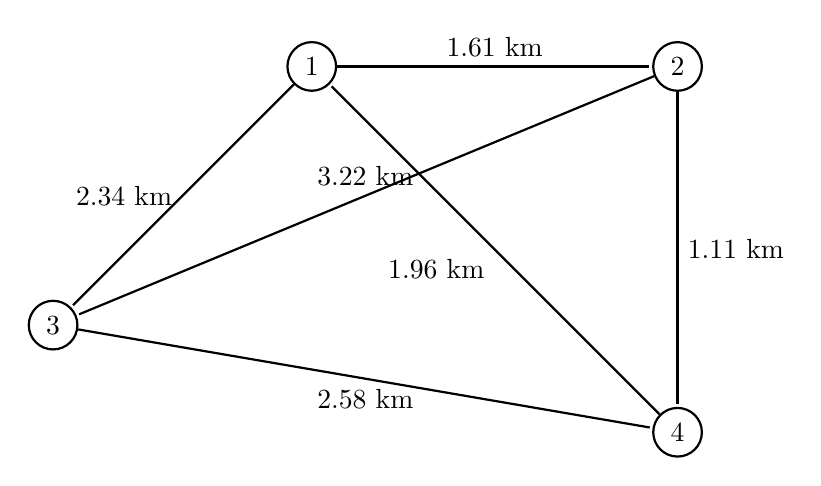
\begin{tikzpicture}[>=stealth,shorten >=1pt,auto,node distance=4cm,thick]
  \node[circle,draw] (1) {1};
  \node[circle,draw,right=of 1] (2) {2};
  \node[circle,draw,below left=of 1] (3) {3};
  \node[circle,draw,below=of 2] (4) {4};
  \path[-,draw] (1) edge node[above] {1.61 km} (2);
  \path[-,draw] (2) edge node[above] {3.22 km} (3);
  \path[-,draw] (3) edge node[below] {2.58 km} (4);
  \path[-,draw] (4) edge node[below left] {1.96 km} (1);
  \path[-,draw] (1) edge node[left] {2.34 km} (3);
  \path[-,draw] (2) edge node[right] {1.11 km} (4);
\end{tikzpicture}
\caption{A Simplified Map}
\end{figure}
\FloatBarrier % Prevent figures from floating past this point

\textbf{3.1.3. Brute Force Approach Analysis} \cite{Bruteforce}
\begin{enumerate}
    \item Represent nodes and paths in the matrix representation (based on Figure 2)\\
    \\
    A matrix representation of a graph of 4 nodes and 6 paths:
     \[
         \bordermatrix{ & node 1 & node 2 & node 3 & node 4\cr
           node 1 & 0 & 1.61 & 2.34 & 1.96\cr
           node 2 & 1.61 & 0 & 3.22 & 1.11\cr
           node 3 & 2.34 & 3.22 & 0 & 2.58\cr
           node 4 & 1.96 & 1.11 & 2.58 & 0} \qquad
     \]

    A total of 6 permutations (branches) in a tree representation:
    \begin{figure}[h]
    \centering
    \begin{forest}
      for tree={
        circle,
        draw,
        minimum size=1.5em,
        s sep=2em,
        l sep=2em,
      }
      [1
        [2, edge label={node[midway,above left] {1.61 km}}
          [3, edge label={node[midway,above left] {3.22 km}}
            [4, edge label={node[midway,above left] {2.58 km}}
              [1, edge label={node[midway,above left] {1.96 km}}, label=below:{\footnotesize sum=9.37 km}]
            ]
            [, phantom]
          ]
          [4, edge label={node[midway,above right] {1.11 km}}
            [, phantom]
            [3, edge label={node[midway,above left] {2.58 km}}
              [1, edge label={node[midway,above left] {2.34 km}}, label=below left:{\footnotesize sum=7.64 km}]
            ]
          ]
        ]
        [3, edge label={node[midway,above right] {2.34 km}}
          [2, edge label={node[midway,above left] {3.22 km}}
            [4, edge label={node[midway,above left] {1.11 km}}
              [1, edge label={node[midway,above right] {1.96 km}}, label=below:{\footnotesize sum=8.63 km}]
            ]
            [, phantom]
          ]
          [4, edge label={node[midway,above right] {2.58 km}}
            [, phantom]
            [2, edge label={node[midway,above left] {1.11 km}}
              [1, edge label={node[midway,above left] {1.61 km}}, label=below left:{\footnotesize sum=7.64 km}]
            ]
          ]
        ]
        [4, edge label={node[midway,above right] {1.96 km}}
          [2, edge label={node[midway,above left] {1.11 km}}
            [3, edge label={node[midway,above right] {3.22 km}}
              [1, edge label={node[midway,above right] {2.34 km}}, label=below:{\footnotesize sum=8.63 km}]
            ]
            [, phantom]
          ]
          [3, edge label={node[midway,above right] {2.58 km}}
            [, phantom]
            [2, edge label={node[midway,above right] {3.22 km}}
              [1, edge label={node[midway,above right] {1.61 km}}, label=below:{\footnotesize sum=9.37 km}]
            ]
          ]
        ]
      ]
    \end{forest}
    \caption{Brute Force Algorithm Analysis for Pokémon Go Routes}
    \end{figure}
    \FloatBarrier % Prevent figures from floating past this point
    \item Calculate total distance for each permutation for every branch of the tree (as shown in Figure 3) \\
    \item Find the minimum distance (e.g. node 1 - node 2 - node 4 - node 3 - node 1 = 7.64 km)
\end{enumerate}
\FloatBarrier % Prevent figures from floating past this point
\textbf{3.1.4. Computation Costs}\\

If n presents the number of nodes, all possible permutations of node orderings is calculated as:
\[(n-1)!\]

For example, when $n = 4, 3! = 3 \times 2 \times 1 = 6$.\\

\textbf{3.1.5. Pros and Cons of Brute Force}\\

Pros
    \begin{enumerate}
        \item Simplicity: it is straightforward to implement, making them suitable for quick solutions and easy understanding.
        \item Guaranteed Solution: it guarantees finding the optimal solution, as it exhaustively explores all possibilities.
    \end{enumerate}

Cons
    \begin{enumerate}
        \item Inefficiency: it is highly inefficient, especially for large input sizes, as they examine all possible solutions without exploiting problem-specific
        \item Computational Complexity: The time and space complexity making it impractical. When $n=11$, there is $3,628,800 (10!)$ permutations.\\
    \end{enumerate}


\subsection{Nearest Neighbor}     % Joshua

\textbf{3.2.1. Overview and Brief History}
\\One of the most common and intuitive solutions is known as the “Nearest neighbour” solution. Starting at an arbitrary point, lines are drawn from each successive point to the one nearest to it, hence the name “nearest neighbour”. 
\\
\\This method was specifically noted by Carl Menger, who studied the travelling salesman problem during the 1930s. The paper “\textit{On the History of Combinatorial Optimization (till 1960)”}, Karl Menger describes the difficulty of the brute-force method and also the lack of an efficient algorithm for a perfect solution, 
\\
\begin{center}
    “\textit{Of course, this problem is solvable by finitely many trials. Rules which would push the number of trials below the number of permutations of the given points, are not known. The rule that one first should go from the starting point to the closest point, then to the point closest to this, etc., in general does not yield the shortest route.}”
\end{center}

\cite{Schrijver1960}


\textbf{3.2.2. Efficiency of Method}

The nearest neighbour method will usually yield a route 25 percent longer than the ideal path for a number of points on a plane. However, specific arrangements might see this method finding a worse, or even the worst possible solution to the problem.
\\
\\This algorithm will usually not find the optimal solution. However, it can and often is used to find a baseline for further improvement by other methods. The nearest neighbour method is notably a “greedy” method, seeking the best short-term outcome for each successive line drawn. Other optimization methods, will sometimes accept worse solutions temporarily to try to find better overall solutions. 
\\
\\One preliminary method to gauge the success of the nearest neighbour method is to compare the length of the first half of the tour to the last half. If the tours are roughly equal in length, then it is likely that the method has given a reasonable baseline. However, if the lengths are not close to equal, then it is likely that the algorithm was too ‘greedy’, sacrificing too much overall efficiency for a better route in the short term. 
\cite{yenigun2023}
\\
\\Note that in the example shown previously, the ideal solution is discovered by the nearest neighbor method, beginning at any of the points, but in a slightly more complex diagram, the method begins to fall apart.
\begin{figure}[h]
\centering
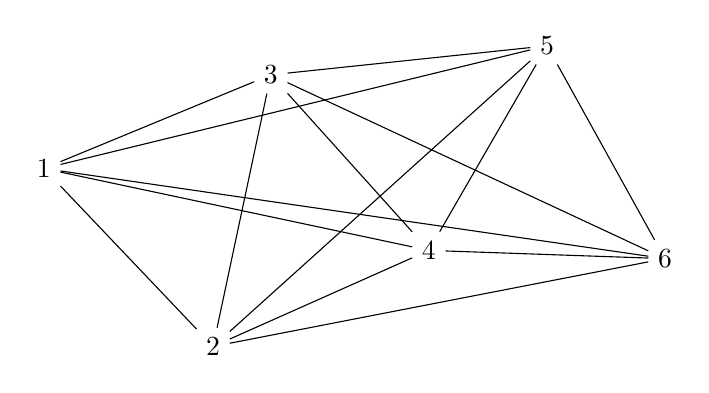
\begin{tikzpicture}
\node(n4) at (0,0){4};
\node(n5) at (60:3){5};
\node(n3) at (132:3){3};
\node(n2) at (204:3){2};
\node(n6) at (358:3){6};
\node(n1) at (168:5){1};
\path[-,draw](n1)--(n2);
\path[-,draw](n1)--(n3);
\path[-,draw](n1)--(n4);
\path[-,draw](n1)--(n5);
\path[-,draw](n1)--(n6);
\path[-,draw](n2)--(n3);
\path[-,draw](n2)--(n4);
\path[-,draw](n2)--(n5);
\path[-,draw](n2)--(n6);
\path[-,draw](n3)--(n4);
\path[-,draw](n3)--(n5);
\path[-,draw](n3)--(n6);
\path[-,draw](n4)--(n5);
\path[-,draw](n4)--(n6);
\path[-,draw](n5)--(n6);
\end{tikzpicture}
\caption{Nearest Neighbor Example}
\end{figure}

\[
         \bordermatrix{ & node 1 & node 2 & node 3 & node 4 & node 5 & node 6\cr
           node 1 & 0 & 2.21 & 2.34 & 3.65 & 4.18 &                 4.78\cr
           node 2 & 2.21 & 0 & 2.67 & 2.12 & 4.06 &                 3.99\cr
           node 3 & 2.34 & 2.67 & 0 & 2.08 & 2.39 &                 3.91\cr
           node 4 & 3.65 & 2.12 & 2.08 & 0 & 2.78 &                 0.97\cr
           node 5 & 4.18 & 4.06 & 2.39 & 2.78 & 0 &                 3.01\cr
           node 6 & 4.78 & 3.99 & 3.91 & 0.97 & 3.01 &              0\cr} \qquad
     \]
\\
\\Use the nearest neighbor method to find a solution, starting from node 3. What is your solution? See if you can find a better one by starting at other nodes or with any other method.
\\
\newpage
\textbf{3.2.3. Further Optimization
\\}One simple method that can be used to immediately shorten a given path is the act of swapping lines that cross over each other. As the figure above shows, this will always yield a better path because of the triangle inequality.
\\\textbf{}
\\\begin{figure}
    \centering
    \includegraphics[width=12cm]{Images/Screenshot 2024-03-06 115708.png}
    \caption{Path swap explanation}
\end{figure}
\\
\\\textbf{Homework Problem}
Take a look at Dantzig 49, one of the first large-scale TSPs that was solved. Look at the map and the distance matrix. Start at a city of your choice and use the nearest neighbor method to find the next 20 cities. Now compare your solution so far to the ideal one found in 1954. Note that only 42 cities are shown out of the original 49, since the solution passed naturally through the 7 cities not listed. You can use this Google Earth project to plot the cities. https://earth.google.com/earth/d/1ElfLqJ7E7alScPKBDwD0J2hwYUdZXutu?usp=sharing
\\
\begin{center}
\begin{tabular}{ c c c }
 1. Manchester & 2. Montpelier & 3. Detroit \\
 4. Cleveland & 5. Charleston & 6. Louisville \\ 
 7. Indianapolis & 8. Chicago & 9. Milwaukee \\
 10. Minneapolis & 11. Pierre & 12. Bismarck \\
 13. Helena & 14. Seattle & 15. Portland \\
 16. Boise & 17. Salt Lake City & 18. Carson City \\
 19. Los Angeles & 20. Phoenix & 21. Santa Fe \\
 22. Denver & 23. Cheyenne & 24. Omaha \\
 25. Des Moines & 26. Kansas City & 27. Topeka \\
 28. Oklahoma City & 29. Dallas & 30. Little Rock \\
 31. Memphis & 32. Jackson & 33. New Orleans \\
 34. Birmingham & 35. Atlanta & 36. Jacksonville \\
 37. Columbia & 38. Raleigh & 39. Richmond \\
 40. Washington D.C. & 41. Boston & 42. Portland
\end{tabular}
\end{center}
\begin{figure}
    \includegraphics[width=17cm]{Images/dfj_table.jpg}
    \caption{Distance Matrix for Dantzig 42}
\end{figure}
\begin{figure}
    \includegraphics[width=12cm]{Images/dantzig_big.jpg}
    \caption{Dantzig 42 optimal solution}
\end{figure}
\subsection{Dynamic Programming}



We have a set of vertices numbered from 1 to n. We want to find the shortest cycle that starts and ends at vertex 1, visiting each vertex exactly once. To do this, we calculate the minimum cost path from vertex 1 to each other vertex, and then add the distance from that vertex back to vertex 1. We repeat this process for each vertex and return the minimum total cost.

To find the cost for each vertex, we use dynamic programming. We define a function C(S, i) as the cost of the minimum path starting at vertex 1, ending at vertex i, and visiting each vertex in set S exactly once. We start by calculating C(S, i) for all subsets S of size 2, then for all subsets of size 3, and so on, until we cover all vertices. In each step, we ensure that vertex 1 is included in the subset.

 \includegraphics[width=10cm]{Images/Euler12.png}
    \label{example}

The python code for this example looks as following:

    \includegraphics[width=12cm]{Images/screenshot TSP project 1.png}

    
    \includegraphics[width=12cm]{Images/screenshot TSP project 2.png}
\cite{Dynamicprogramming}
    

\section{Modern Day Scenarios}  % Kirollos
\subsection{Transportation}
The traveling salesman problem (TSP) is extremely useful in the modern-day, with its most obvious use case being for companies in the transportation industry. These companies often need to deliver products to several places in the most efficient way, both to save on energy consumption and for customer convenience. \cite{Optessa}

\subsection{Telecommunications}        
Another important use case for the TSP is in the telecommunications industry. To best satisfy customers, telecommunications companies need to implement their stations in such a way as to provide network access to the most amount of people while still retaining a high-performance connection. \cite{Optessa}
\subsection{Manufacturing}
The TSP is additionally useful for manufacturers. In factories, machines are arranged in a way that allows for a worker to quickly reach one in case it needs maintenance; having the shortest possible distance between all parts of the production line allows for the factory to be most productive, as less time is wasted on fixing it. \cite{Optessa}

\subsection{Bio-engineering}    
The traveling salesman problem is also important in biology, specifically in dealing with DNA sequencing.  When gathering DNA fragments, scientists can use the TSP to figure out how to reconstruct them back to their original sequence.
\cite{Optessa}
\subsection{Robotics}     
Recently, there has been an influx of use cases for the TSP in machinery. For instance, self-driving cars require knowledge of the most optimal paths on the road to maximize efficiency. Moreover, robots such as Roombas need to be able to move most efficiently in a given area to conserve energy. \cite{Optessa}

\newpage
\section{Sources Cited}
\printbibliography
https://www.math.uwaterloo.ca/tsp/history/index.html
\end{document}
